\documentclass[a4paper, 12pt]{article}
\usepackage[a4paper,top=1.5cm, bottom=1.5cm, left=1cm, right=1cm]{geometry}
\usepackage{cmap}					
\usepackage{mathtext} 				
\usepackage[T2A]{fontenc}			
\usepackage[utf8]{inputenc}			
\usepackage[english,russian]{babel}
\usepackage{multirow}
\usepackage{graphicx}
\usepackage{wrapfig}
\usepackage{tabularx}
\usepackage{float}
\usepackage{longtable}
\usepackage{hyperref}
\hypersetup{colorlinks=true,urlcolor=blue}
\usepackage[rgb]{xcolor}
\usepackage{amsmath,amsfonts,amssymb,amsthm,mathtools} 
\usepackage{icomma} 
\usepackage{euscript}
\usepackage{mathrsfs}
\usepackage{enumerate}
\usepackage{caption}
\usepackage{enumerate}
\mathtoolsset{showonlyrefs=true}
\usepackage{graphicx}
\usepackage{caption}
\usepackage{subcaption}
\usepackage{amsthm}
\usepackage[europeanresistors, americaninductors]{circuitikz}
\DeclareMathOperator{\sgn}{\mathop{sgn}}
\newcommand*{\hm}[1]{#1\nobreak\discretionary{}
	{\hbox{$\mathsurround=0pt #1$}}{}}

\title{\textbf{Получение и измерение вакуума (2.3.1)}}
\author{Манро Эйден}
\date{}

\begin{document}

\maketitle

\begin{center}
    \section*{Введение}
\end{center}

    \noindent \textbf{Цель работы:} 1) измерение объемов форвакуумной и высоковакуумной частей установки; 2) определение скорости откачки системы в стационарном режиме, а такжепо ухудшению и улучшению вакуума.

    \bigskip

    \noindent \textbf{Оборудование:} вакуумная установка с манометрами: масляным, термопарным и ионизационным. В данной работе используются традиционные методы откачки механическим форвакуумным насосом до давления $10^{-2}$ торр и диффузионным масляным насосом до давления $10^{-4}$ торр. 

    \bigskip

\begin{center}
    \section*{Теоретические сведения}
\end{center}

  
\subsection*{Процесс откачки}

Опишем процесс откачки математически: 
Пусть W --- объем газа, удаляемого из сосуда при данном давлении за единицу времени, $Q_i$ для различных значений $i$ обозначим различные притоки газа в сосуд (в единицах $PV$), такие как течи извне $Q_\text{и}$, десорбция с поверхностей внутри сосуда $Q_\text{д}$, обратный ток через насос $Q_\text{н}$. Тогда, приравнивая убыль газа из сосуда (с точностью до $RT/\mu$) в единицу времени $-VdP$ и сумму перечисленных токов имеем:

\bigskip

\begin{equation}
    -VdP = (PW - \sum_i Q_i)dt
\end{equation}

\bigskip

При достижении предельного вакуума устанавливается давление $P_{\text{пр}}$, и $dP = 0$. Тогда

\bigskip

\begin{equation}
 	W = \frac{ \sum_i Q_i }{P_{\text{пр}}}
\end{equation}

\bigskip

Поскольку обычно $Q_\text{и}$ постоянно, а $Q_\text{н}$ и $Q_\text{д}$ слабо зависят от времени, также считая постоянной W, можем проинтегрировать (1) и получить:

\bigskip

\begin{equation}
 	P - P_{\text{пр}} = (P_0 - P_{\text{пр}})\exp(-\frac{W}{V}t)
\end{equation}

\bigskip

Полная скорость откачки $W$, собственная скорость откачки насоса $W_{\text{н}}$ и проводимости элементов системы $C_1, C_2,...$ соотносятся согласно формуле (4), и это учтено в конструкции установки.

\bigskip

\begin{equation}
    \frac{1}{W} = \frac{1}{W} + \frac{1}{C_1} + \frac{1}{C_2} + ...
\end{equation}

\subsection*{Течение газа через трубу}

Характер течения газа существенно зависит от соотношения между размерами системы и длиной свободного пробега молекул. При атмосферном и форвакуумном давлениях  длина свободного пробега меньше диаметра трубок, и течение газа определяется его вязкостью, т.е. взаимодействием молекул. При высоком вакууме течение существеннее определяется взаимодействием со стенками \\
Для количества газа, протекающего через трубу длины $l$ и радиуса $r$ в условиях высокого вакуума, справедлива формула:

\bigskip

\begin{equation}
	\frac{d(PV)}{dt} = \frac{4}{3}r^3\sqrt{\frac{2\pi RT}{\mu}}\frac{P_2 - P_1}{l}
\end{equation}

\bigskip

Если труба соединяет насос установку, то давлением $P_1$ у насоса можно пренебречь. Давление в сосуде $P = P_2$. Тогда имеем:

\bigskip

\begin{equation}
    C_\text{тр} = \left(\frac{dV}{dt}\right)_\text{тр} = \frac{4r^3}{3l}\sqrt{\frac{2\pi RT}{\mu}}
\end{equation}


\subsection*{Экспериментальная установка}

\; \; Установка изготовлена из стекла,
и состоит из форвакуумного баллона (ФБ), высоковакуумного диффузионного насоса (ВН), высоковакуумного баллона (ВБ), масляного (М) и ионизационного (И) манометров, термопарных манометров ($\text{М}_1$ и $\text{М}_2$), форвакуумного насоса (ФН) и соединительных кранов ($К_1, К_2,..., К_6$) (Рис. 1). Кроме того, в состав установки входят: вариатор (автотрансформатор с регулируемым выходным напряжением), или реостат и амперметр для регулирования тока нагревателя диффузионного насоса.

\begin{figure}[H]
 	\centering
 	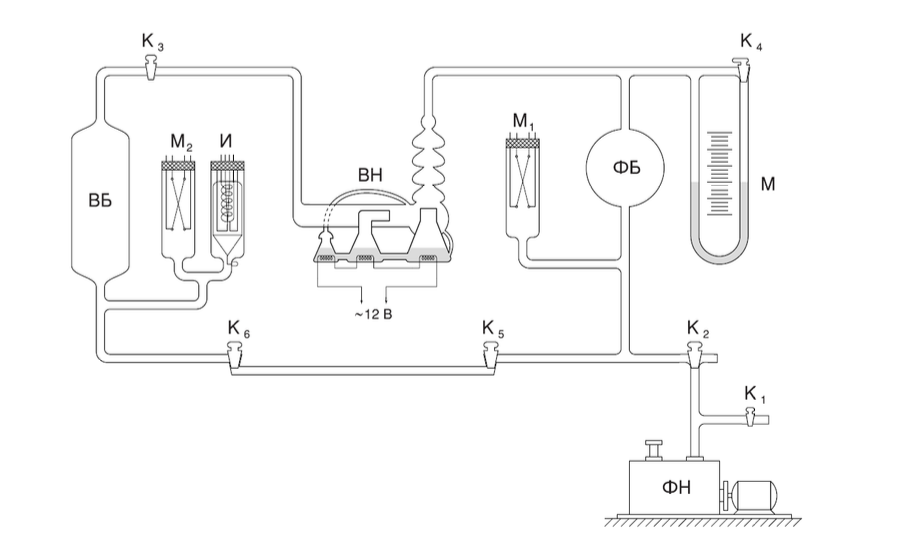
\includegraphics[width=0.7 \textheight]{1.jpg}
 	\caption{Схема установки}
 	\label{fig:Схема установки}
\end{figure}

Кран $К_1$ используется для заполнения форвакуумного насоса и вакуумной установки атмосферным воздухом. Во время работы установки
он должен быть закрыт. Трёхходовой кран $К_2$ служит для соединения
форвакуумного насоса с установкой или атмосферой. Кран $К_3$ отделяет
высоковакуумную часть установки от форвакуумной. Кран $К_4$ соединяет между собой колена масляного манометра. Он должен быть открыт во все время работы установки и закрывается лишь при измерении
давления в форвакуумной части. Краны $К_5$ и $К_6$ стоят по концам капилляра и соединяют его с форвакуумной и высоковакуумной частями установки. 

\begin{figure}[H]
	\centering
	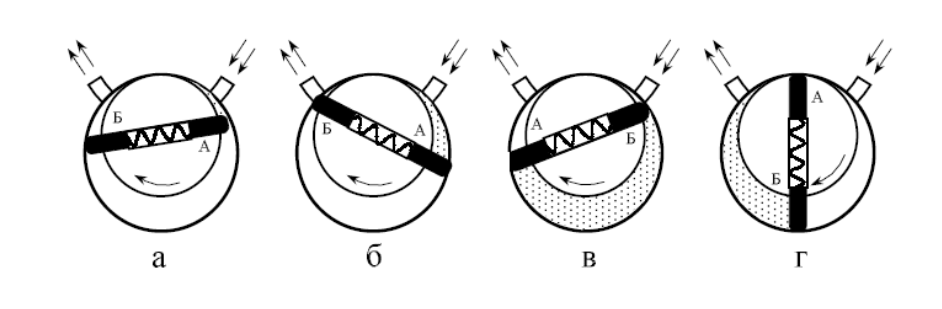
\includegraphics[width=0.9\linewidth]{2.jpg}
	\caption[]{Схема действия ротационного двухпластинчатого форвакуумного насоса}
	\label{fig:Схема ФВ насоса}
\end{figure}

\begin{figure}[H] 
	\centering 
	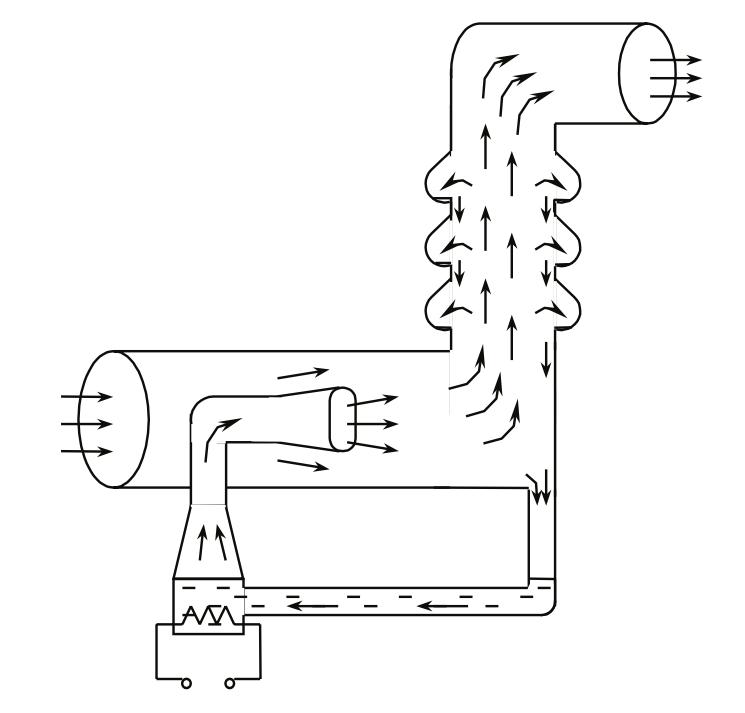
\includegraphics[scale=0.2]{3.jpg} 
	\caption{Схема работы одной ступени диффузионного насоса} 
\end{figure}

Устройство одной ступени масляного диффузионного насоса схематически показано на Рис. 3 (в лабораторной установке используется несколько откачивающих ступеней). Масло, налитое в сосуд, подогревается электрической печкой. Пары масла поднимаются по трубе и вырываются из сопла. Струя паров увлекает молекулы газа, которые поступают из откачиваемого сосуда через трубку. Дальше смесь попадает в вертикальную трубу. Здесь масло осаждается на стенках трубы и маслосборников и стекает вниз, а оставшийся газ откачивается форвакуумным насосом. 

\bigskip

\newpage

\begin{center}
	\subsection*{Погрешности}
\end{center}

\begin{itemize}
	\item $\sigma_{\text{лин}} \; = \; 0,05 \; \text{см}, \; \sigma_{\Delta h} = 0,01 \; \text{см}, \; \sigma_{\rho} = 0,001 \; \frac{\text{г}}{\text{см}^3}, \; \sigma_{V_{\text{зап}}} = 1 \; \text{см}^3, \; \sigma_g = 0,01 \; \frac{\text{м}}{\text{с}^2} $
	\item $\sigma_V = \sqrt{(\frac{\sigma_\rho}{\rho})^2 + (\frac{\sigma_{\Delta h}}{\Delta h})^2 + (\frac{\sigma_{g}}{g})^2 + (\frac{\sigma_{V_\text{зап}}}{V_\text{зап}})^2} $
\end{itemize}

\begin{center}
    \section*{Ход работы}
\end{center}


\subsection*{Входные данные}

\bigskip

\begin{itemize}
	\item $P_\text{атм} = (100140 \pm 400) \; \text{Па}, \; t_\text{к} = (22,9 \pm 0,1) \; ^\circ C, \; \rho_\text{м} = (0,885 \pm 0,001) \; \frac{\text{г}}{\text{см}^3}, \; V_\text{зап} = (50 \pm 1) \; \text{см}^3  $
	\item $L = 10,8 \; \text{см}, \; d = 0,8 \; \text{мм}$
\end{itemize}

Открываем все краны и запускаем в систему воздух из атмосферы ($P_{\text{атм}}$). Закрываем краны $К_5$ и $К_6$, тем самым заперев в кранах и в капилляре воздух объемом ($V_{\text{зап}}$). Откачиваем воздух из системы при помощи форвакуумного насоса. После откачки до давления $\sim 10^{-2} торр$ запираем кран 2 и изолируем систему от атмосферы. Закрывая кран у масляного манометра приводим его в рабочее состояние. Отсакаем высоковакуумную часть закрытием крана 3 и впускаем запертый в кране 5 воздух в форвакуумную часть установки. при этом, давление в форвакуумной части возрастает, о чем свидетельствует маслянный манометр. Измеряем давление при помощи последнего и следующим шагом открываем кран 3, соединяя высоковакуумную часть с остальной. При этом давление падает. По этим данным считаем объем высоковакуумной части пользуясь законом Бойля-Мариотта. Заметим, что здесь мы пренебрегли начальным давлением (порядка $\sim 10^{-2} торр$) т.к. оно в $\sim 1000$ раз меньше других давлении.

\bigskip

\begin{equation}
	P_{\text{атм}}V_{\text{зап}}=P_1V_{\text{фв}}=P_2(V_{\text{фв}}+V_{\text{вв}})
\end{equation}

Измеренные давления:


\begin{align}
	\Delta h_1=(26,3 \pm 0,1) \; \text{см} \\
	\Delta h_2=(17,1 \pm 0,1) \; \text{см} \\
\end{align}

Подставляя получаем:

\begin{align}
	V_{\text{фв}} &= (2192 \pm 45) \; \text{см}^3, \; \varepsilon_{\text{фв}} = 2 \; \% \\
	V_{\text{вв}} &= (1180 \pm 35) \; \text{см}^3, \; \varepsilon_{\text{вв}} = 3 \; \% \\
\end{align}

\subsection*{Получение высокого вакуума и измерение скорости откачки}

Открываем все краны и проводим первоначальную выкачку воздуха форвакуумным насосом. После приближения к предельному давлению ($\sim 10^{-2}торр$), закрываем кран 6 и включаем диффузионный насос. Ждем пока масло закипит и начнется дальнейшая выкачка уже диффузионным насосом. По достижению давления порядка $\sim 10^{-3}торр$ включаем ионизационный манометр, которым и будем измерять давление в дальнейшем.

Чтобы измерить скорость откачки $W$ замерим как изменяется давление в высоковакуумной части от времени. Сосгласно теории давление должно падать по правилу, где у нас $P_{\text{пр}}=5,5\cdot10^{-5} \; \text{торр}$

\begin{equation}
    P-P_{\text{пр}}=(P_0 - P_{\text{пр}})\exp\left(-\frac{W}{V_{\text{вв}}}t\right)
\end{equation}

Логарифмируя, получаем:

\begin{equation}
    \ln(P-P_{\text{пр}})=-\frac{W}{V_{\text{вв}}}t + c
    \label{linearized}
\end{equation}

Аппроксимируя наши данные согласно формуле (\ref{linearized}) получим значение для $W$. Измерение проведем 2 раза. Результаты изображены на графиках \ref{ris:ccum} (данные предоставлены в таблице \ref{plot_data}). Учитывая что погрешности логарифмов растут со временем, и зависимость теряет характерный линейный вид, линеяная аппроксимация была сделана только для оранжевых точек. Пользуясь объемом высоковакуумной части из формулы (7) и данными аппроксимации получаем следующие значения для скорости откачки:


\begin{equation}
	W_1 = (248 \pm 11) \; \frac{\text{см}^3}{\text{с}}, \; \; \; W_2 = (262 \pm 8) \; \frac{\text{см}^3}{\text{с}}
	\label{W_znach}
\end{equation}

Как видим, значеня лежат в пределах погрешности, чего и следовало ожидать.

Теперь определим величину потока $Q_\text{н}$. Для обшего потока имеем формулу
\begin{equation}
	P_{\text{пр}}W = (Q^\prime + Q_\text{н})RT
	\label{Q_nasos}
\end{equation}

где $Q^\prime=Q_\text{и}+Q_\text{д}$. Теперь, если по достижению предельного давления закрыть кран 3, то насос будет отсоиденен от высоковакуумной части, и уравнение описывающее давление от времени примет вид

    \begin{equation*}
        V_{\text{вв}}dP = QRTdt
    \end{equation*}
    интегрируя которую получим
    \begin{equation}
        P = \frac{QRT}{V_{\text{вв}}}t + c
    \end{equation}
    Измерив зависимость давления от времени и аппроксимируя данные прямой можно получить $Q$. Графики приведены на рисунке \ref{ris:cccnum}. Отсюда получаем
    \begin{equation}
        Q_1RT=(65 \pm 6)\cdot 10^{-4} \; \text{торр}\cdot \text{см}^3\text{с}^{-1}, \; Q_2RT=(60 \pm 5)\cdot 10^{-4} \; \text{торр}\cdot\text{см}^3\text{с}^{-1}
    \end{equation}
    Опять же, значения совпадают в пределах погрешности, как и ожидалось. Теперь, используя значения $W_1, W_2, Q_1, Q_2$ по формуле (\ref{Q_nasos}) считаем значение $Q_{н}$
    \begin{equation}
        Q_\text{н}=(0,72 \pm 0,08)\cdot10^{-5} \; \frac{\text{торр} \cdot \text{л}}{\text{с}}
    \end{equation}

	Для $W$ получаем:
    \begin{equation}
    W=\frac{4}{3}\frac{r^3}{L}\sqrt{\frac{2\pi RT}{\mu}}\frac{P_{\text{фв}} - P_{\text{уст}}}{{P_\text{уст}} - P_{\text{пр}}}=(290 \pm 10)\frac{\text{см}^3}{\text{с}}
    \end{equation}

\begin{center}
	$ P_\text{пр} = (5,5 \pm 0,1) \cdot 10^{-5} \; \text{торр} $ \\
	$ P_\text{уст} = (1,3 \pm 0,1) \cdot 10^{-4} \; \text{торр} $ \\
	$ P_\text{фв} = (3,8 \pm 0,1) \cdot 10^{-3} \; \text{торр} $ \\
\end{center}	


	\newpage

	\begin{center}
		\section*{Обсуждение результатов}
	\end{center}
		
	Итак, в ходе данной лабораторной работы нам удалось получить высокий вакуум ($P = 5,5 \cdot 10^{-5}$ торр) с помощью диффузионного и форвакуумного насосов. Рассчитали скорость откачки насоса двумя независимыми способами: по улучшению вакуума и по скорости течения газа через трубу в условиях высокого вакуума. Результаты отличаются менее чем на 5\%, поэтому можно утверждать, что они совпадают в пределах погрешности. 
	
	Вакуум необходим для получения тонких магнитных пленок. Важнейшей областью применения магнитных пленок является их использование для записи и хранения информации в запоминающих устройствах. Для увеличения плотности записи в магнитных пленках намагниченность ориентируют перпендикулярно плоскости пленок. Перпендикулярная ориентация намагниченности в тонких пленках энергетически невыгодна. Сильная перпендикулярная анизотропия в магнитных пленках возможна только при определенных условиях: толщина магнитного материала должна быть не выше критической и магнитный материал должен быть ограничен слоями некоторых тяжелых металлов (Pd, Pt, Ru). Именно граничные слои наводят перпендикулярную анизотропию во всей магнитной пленке. Напыление магнитного материала и тяжелых металлов, например, кобальта ($Co$) и ($Pd$) на кремниевую подложку ($SiO_2$) возможно только в сверхвысоком вакууме.
	
	
	\begin{center}
	    \section*{Выводы}
	\end{center}

	В ходе работы было измерено скорость откачки диффузионного насоса двумя способами
    \begin{equation}
        W_{1} = (248 \pm 11) \; \frac{\text{см}^3}{\text{с}}, \; W_{2} = (262 \pm 8)\; \frac{\text{см}^3}{\text{с}}, \; W = (290 \pm 10)\; \frac{\text{см}^3}{\text{с}}
    \end{equation}
    Значения совпадают в пределах погрешности. Погрешность значения измеренной методом создания исскуственной течи большая в связи с наличием разности двух близких величин в формуле подсчета($P_{уст} - P_{пр}$).

    Во время работы так же было проверенно справедливость отношения
    \begin{equation*}
        P-P_{пр}=(P_0 - P_{пр})\exp\left(-\frac{W}{V}t\right)
    \end{equation*}
    при откачке воздуха и отношения
    \begin{equation*}
        P = \frac{QRT}{V_{вв}}t + c
    \end{equation*}
    описывающее рост давления при отключении насоса от системы.

	\newpage

    \begin{figure}[H]
        \centerline{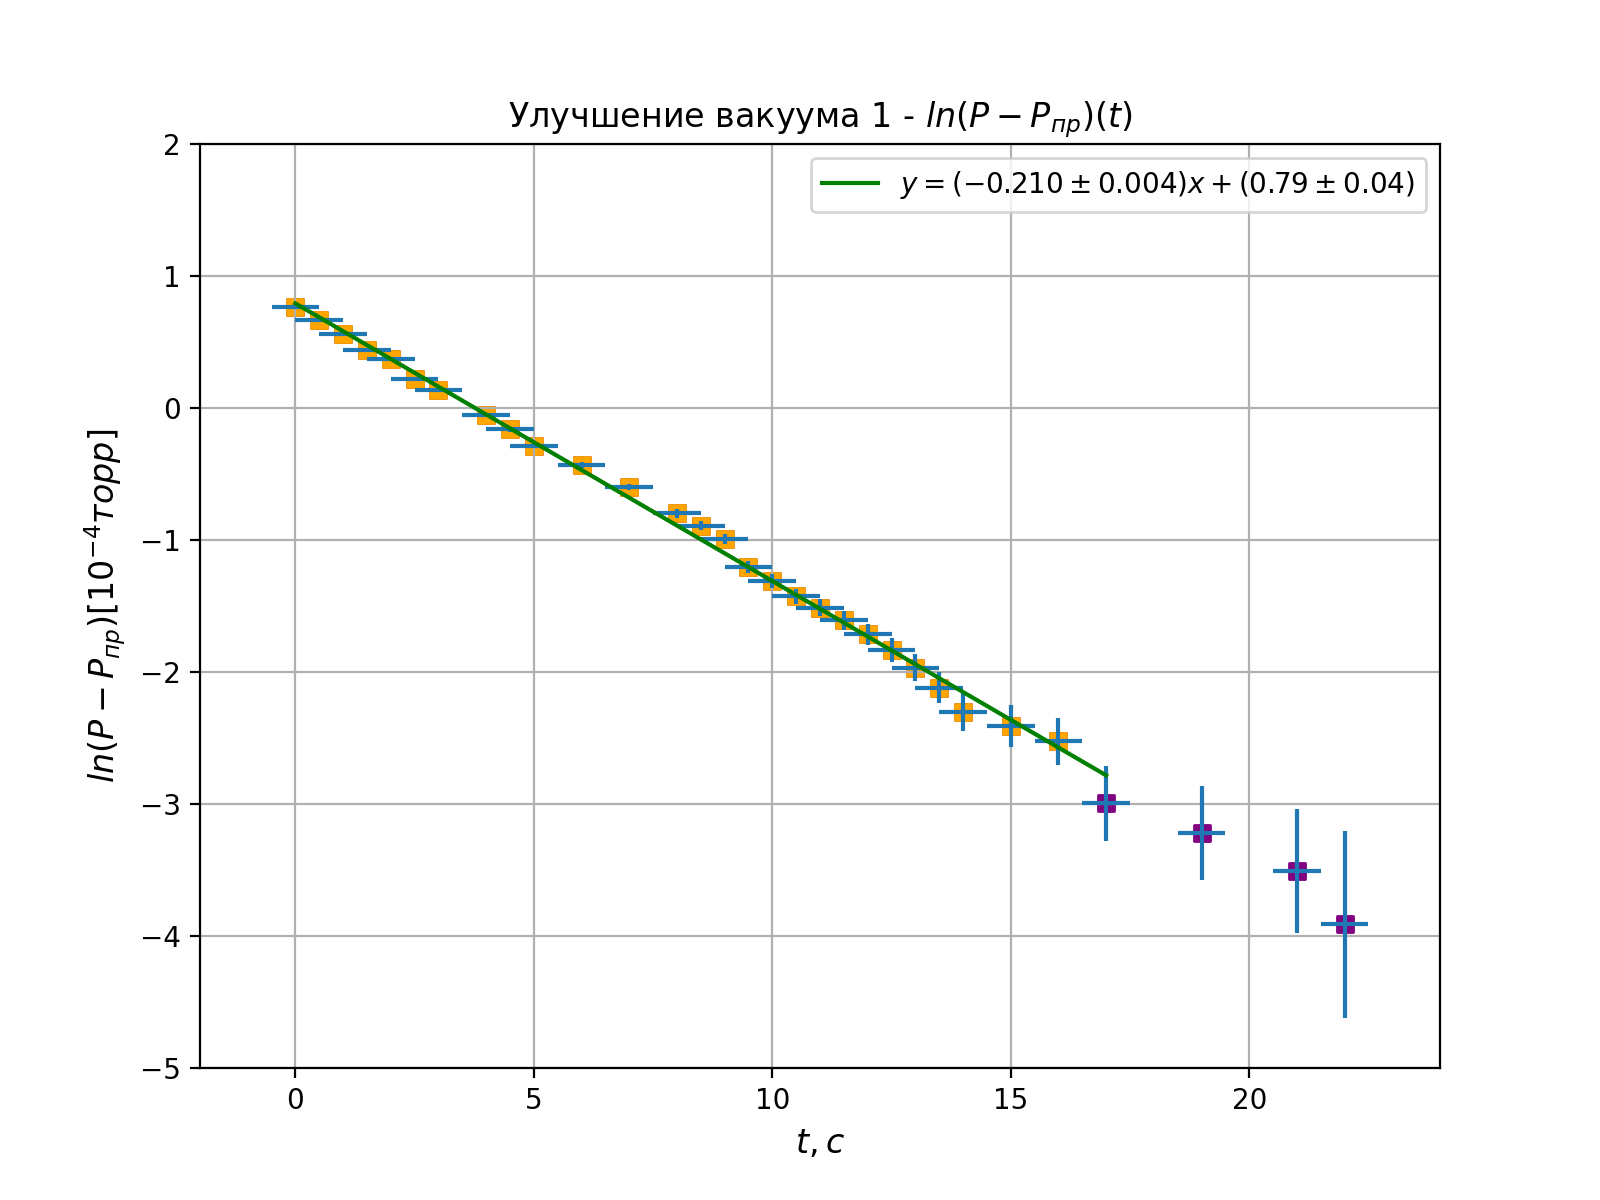
\includegraphics[width=0.8\textwidth]{pictures/ccum_1.png}}
    \end{figure}
    \begin{figure}[H]
        \centerline{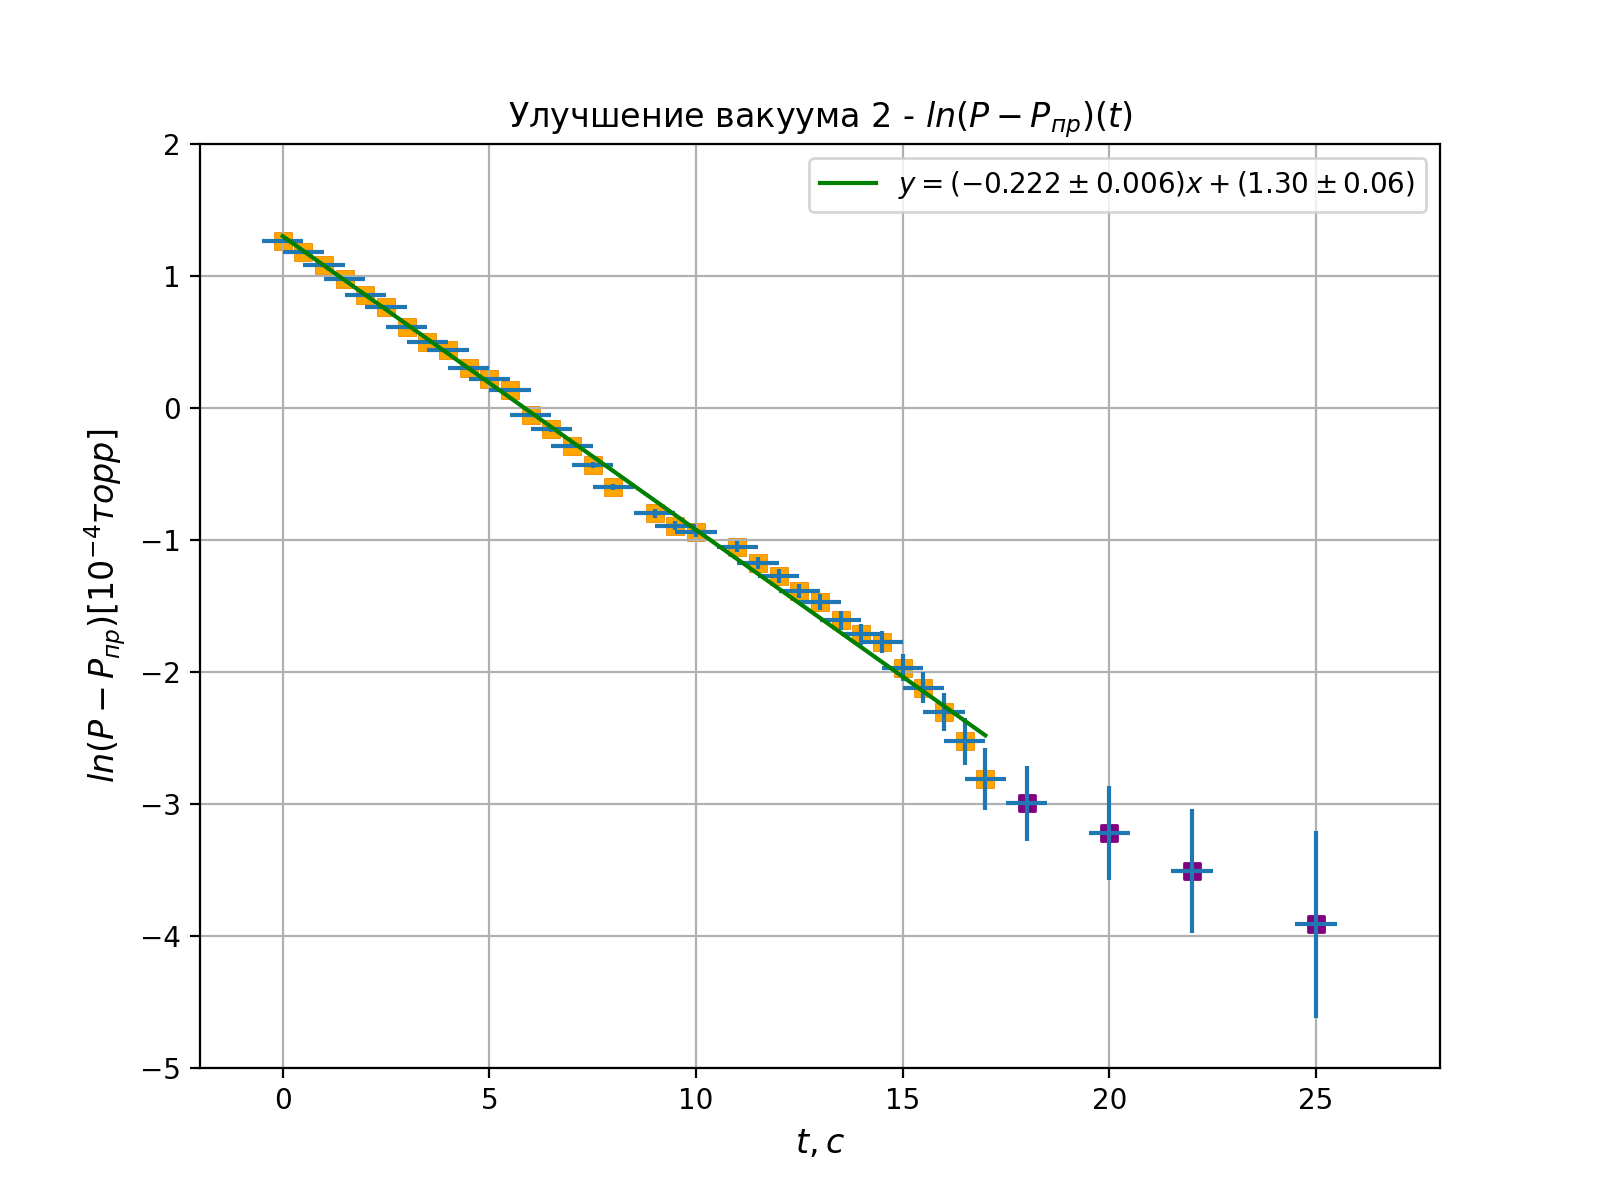
\includegraphics[width=0.8\textwidth]{pictures/ccum_2.png}}
        \caption{Линеаризованные графики улучшения вакуума.}
        \label{ris:ccum}
    \end{figure}

    \newpage
 	
\begin{table}[!h]
    \begin{center}
    \begin{tabular}{rr|rr|rr|rr}
    \toprule
    \multicolumn{2}{c|}{Улучшение 1} & \multicolumn{2}{c|}{Улучшение 2} & \multicolumn{2}{c|}{Ухудшение 1} & \multicolumn{2}{c}{Ухудшение 2}\\
    $t, с$ &  $P, 10^{-4}торр$ & $t, с$ &  $P, 10^{-4}торр$ & $t, с$ &  $P, 10^{-4}торр$ & $t, с$ &  $P, 10^{-4}торр$\\
    \midrule

	0.00 & 5.60 & 0.00 & 6.00 & 0 & 1.00 & 0 & 1.00 \\
	0.50 & 5.30 & 0.50 & 5.90 & 2 & 1.10 & 1 & 1.10 \\
	1.00 & 5.00 & 1.00 & 5.70 & 3 & 1.20 & 3 & 1.20 \\
	1.50 & 4.60 & 1.50 & 5.60 & 5 & 1.30 & 5 & 1.30 \\
	2.00 & 4.30 & 2.00 & 5.30 & 7 & 1.40 & 7 & 1.40 \\
	2.50 & 3.60 & 2.50 & 5.10 & 9 & 1.50 & 9 & 1.50 \\
	3.00 & 3.20 & 3.00 & 4.80 & 11 & 1.60 & 12 & 1.60 \\
	3.50 & 3.00 & 3.50 & 4.40 & 12 & 1.70 & 14 & 1.70 \\
	0.00 & 2.70 & 0.00 & 4.10 & 14 & 1.80 & 16 & 1.80 \\
	0.50 & 2.50 & 0.50 & 3.80 & 15 & 1.90 & 19 & 1.90 \\
	1.00 & 2.30 & 1.00 & 3.50 & 17 & 2.00 & 21 & 2.00 \\
	1.50 & 2.10 & 1.50 & 3.20 & 19 & 2.10 & 23 & 2.10 \\
	2.00 & 2.00 & 2.00 & 2.90 & 21 & 2.20 & 26 & 2.20 \\
	2.50 & 1.80 & 2.50 & 2.70 & 23 & 2.30 & 28 & 2.30 \\
	3.00 & 1.70 & 3.00 & 2.40 & 25 & 2.40 & 30 & 2.40 \\
	4.00 & 1.50 & 3.50 & 2.20 & 27 & 2.50 & 31 & 2.50 \\
	4.50 & 1.40 & 4.00 & 2.10 & 29 & 2.60 & 33 & 2.60 \\
	5.00 & 1.30 & 4.50 & 1.90 & 30 & 2.70 & 35 & 2.70 \\
	6.00 & 1.20 & 5.00 & 1.80 & 32 & 2.80 & 38 & 2.80 \\
	7.00 & 1.10 & 5.50 & 1.70 & 34 & 2.90 & 40 & 2.90 \\
	8.00 & 1.00 & 6.00 & 1.50 & 35 & 3.00 & 41 & 3.00 \\
	8.50 & 0.96 & 6.50 & 1.40 & 37 & 3.10 & 43 & 3.10 \\
	9.00 & 0.92 & 7.00 & 1.30 & 39 & 3.20 & 45 & 3.20 \\
	9.50 & 0.85 & 7.50 & 1.20 & 41 & 3.30 & 47 & 3.30 \\
	10.00 & 0.82 & 8.00 & 1.10 & 43 & 3.40 & 49 & 3.40 \\
	10.50 & 0.79 & 9.00 & 1.00 & 45 & 3.50 & 51 & 3.50 \\
	11.00 & 0.77 & 9.50 & 0.96 & 47 & 3.60 & 52 & 3.60 \\
	11.50 & 0.75 & 10.00 & 0.94 & 49 & 3.70 & 54 & 3.70 \\
	12.00 & 0.73 & 11.00 & 0.90 & 50 & 3.80 & 56 & 3.80 \\
	12.50 & 0.71 & 11.50 & 0.86 & 51 & 3.90 & 58 & 3.90 \\
	13.00 & 0.69 & 12.00 & 0.83 & 53 & 4.00 & 60 & 4.00 \\
	13.50 & 0.67 & 12.50 & 0.80 & 55 & 4.10 & 62 & 4.10 \\
	14.00 & 0.65 & 13.00 & 0.78 & 57 & 4.20 & 64 & 4.20 \\
	15.00 & 0.64 & 13.50 & 0.75 & 59 & 4.30 & 66 & 4.30 \\
	16.00 & 0.63 & 14.00 & 0.73 & 60 & 4.40 & 68 & 4.40 \\
	17.00 & 0.60 & 14.50 & 0.72 & 62 & 4.50 & 70 & 4.50 \\
	19.00 & 0.59 & 15.00 & 0.69 & 65 & 4.60 & 72 & 4.60 \\
	21.00 & 0.58 & 15.50 & 0.67 & 66 & 4.70 & 74 & 4.70 \\
	22.00 & 0.57 & 16.00 & 0.65 & 68 & 4.80 & 76 & 4.80 \\
	25.00 & 0.56 & 16.50 & 0.63 & 70 & 4.90 & 78 & 4.90 \\
\bottomrule
\end{tabular}
\end{center}
\caption{Данные для построения графиков}
\label{plot_data}
\end{table}

    \begin{figure}[h]
        \centerline{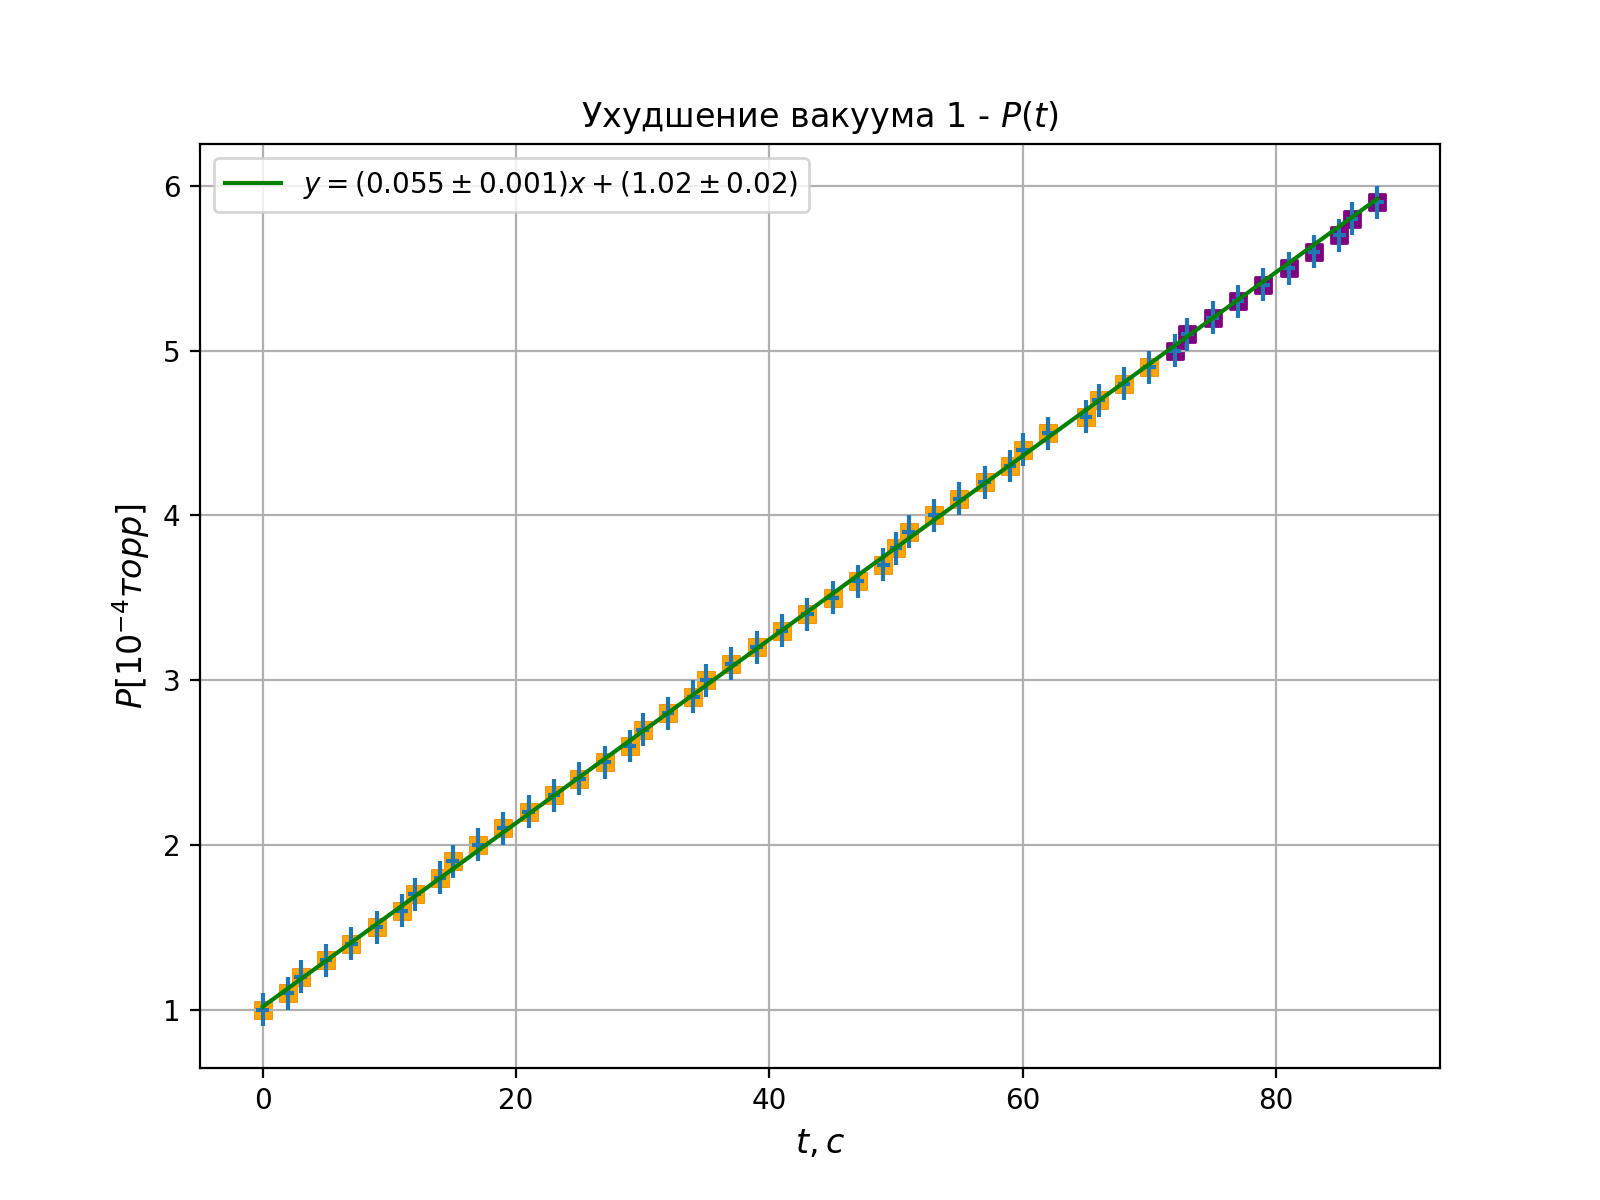
\includegraphics[width=0.9\textwidth]{pictures/cccnum_1.png}}
        \centerline{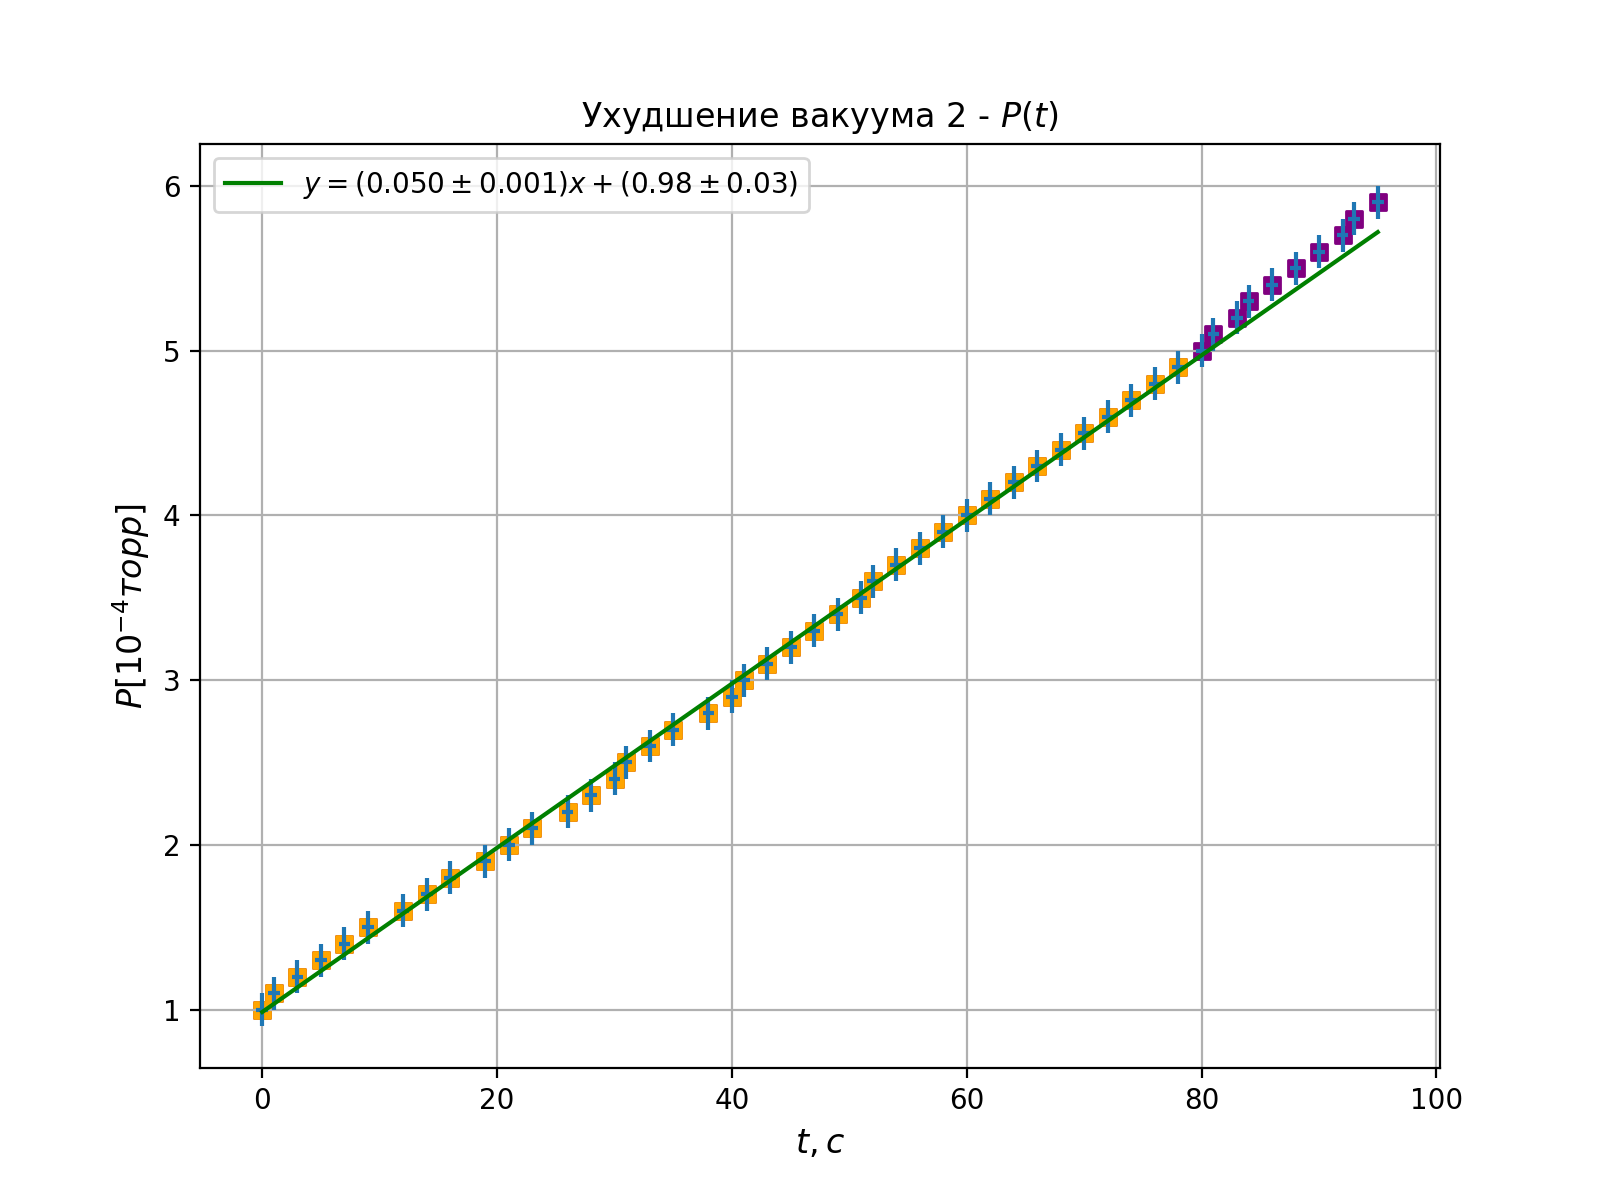
\includegraphics[width=0.9\textwidth]{pictures/cccnum_2.png}}
        \caption{Графики ухудшения вакуума.}
        \label{ris:cccnum}
    \end{figure}



\end{document}